\chapter{Schlussfolgerung}

\section{Ergebnis}
Wenn wir unsere Programm auführen erhalten wir folgende Ausgabe:

\begin{figure}[h]
    \begin{center}
        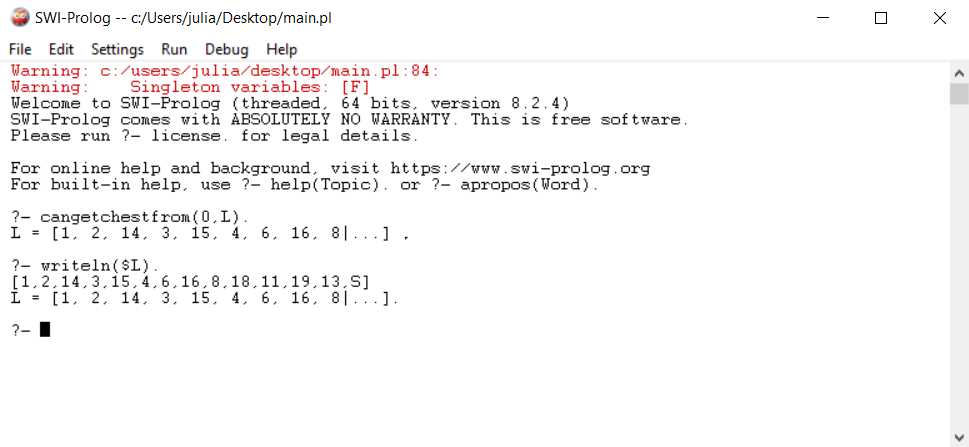
\includegraphics[width=1\textwidth]{content/pictures/output.png}
        \caption{Output Prolog Keys and Doors}
        \label{fig:output}
    \end{center}
\end{figure}

\noindent
Wie auf der Abbildung zu erkennen ist, braucht der Agent genau 13 Schritte bis
er beim Schatz angekommen ist. Dies ist nur eine von mehreren Lösungen, welche 
das Programm haben könnte.

\section{Fazit}
Es war interessant einmal mit einer Sprache zu programmieren, in welcher nicht alle
bereits bekannten Konzepte wie Listen oder Variabeln implementiert waren. Dadurch mussten 
diese einfachste Dinge wie Loops selbst umgesetzt werden. Dies hat uns etwas mehr Zeit gekostet
als wir es gedacht hatten. Zudem war es interessant die Vielfalt von Prolog kennen zu lernen.
Die Sprache hat ihre Eigenheiten und muss zuerst gut kennengelernt werden, bevor man mit der
Programmierung beginnt.  